\documentclass[a4paper,14pt]{extarticle}
\usepackage[a4paper,top=1.3cm,bottom=2cm,left=1.5cm,right=1.5cm,marginparwidth=0.75cm]{geometry}
\usepackage{setspace}
\usepackage{cmap}					
\usepackage{mathtext} 				
\usepackage[T2A]{fontenc}			
\usepackage[utf8]{inputenc}			
\usepackage[english,russian]{babel}
\usepackage{multirow}
\usepackage{graphicx}
\usepackage{wrapfig}
\usepackage{tabularx}
\usepackage{float}
\usepackage{longtable}
\usepackage{hyperref}
\hypersetup{colorlinks=true,urlcolor=blue}
\usepackage[rgb]{xcolor}
\usepackage{amsmath,amsfonts,amssymb,amsthm,mathtools} 
\usepackage{icomma} 
\mathtoolsset{showonlyrefs=true}
\usepackage{euscript}
\usepackage{mathrsfs}

\DeclareMathOperator{\sgn}{\mathop{sgn}}
\newcommand*{\hm}[1]{#1\nobreak\discretionary{}
	{\hbox{$\mathsurround=0pt #1$}}{}}

\newcommand{\RomanNumeralCaps}[1]
{\MakeUppercase{\romannumeral #1}}

\usepackage{soulutf8} 
\usepackage{geometry}



\begin{document}
	\begin{center}
		\textit{Федеральное государственное автономное образовательное\\ учреждение высшего образования }
		
		\vspace{0.5ex}
		
		\textbf{«Московский физико-технический институт\\ (национальный исследовательский университет)»}
	\end{center}
	
	\vspace{10ex}
	
	
	\begin{center}
		\vspace{13ex}	
		\textbf{Лабораторная работа №1.2.3}	
		\vspace{1ex}
		
		по курсу общей физики		
		на тему:		
		\textbf{\textit{<<Определение момента инерции твердых тел с помощью трифилярного подвеса>>}}		
		\vspace{30ex}
		
		\begin{flushright}
			\noindent
			\textit{Работу выполнил:}\\  
			\textit{Никифоров Дмитрий \\(группа Б02-205)}
		\end{flushright}
		\vfill
		Долгопрудный \\ \today
		
		%\setcounter{page}{1}
	\end{center}
	\newpage
	
	\section{Введение}
	
	\textbf{Цель работы:} исследовать прецессию уравновешенного гироскопа, установить зависимость скорости вынужденной прецессии от величины момента сил, действующий на ось гироскопа и сравнить ее со скоростью, рассчитанной по скорости прецессии; определить скорость вращения ротора гироскопа и сравнить со значением частоты вращения, полученным при помощи осциллографа.\\
	\textbf{Оборудование:} гироскоп в кардановом подвесе, секундомер, набор грузов, отдельный ротор гироскопа, цилиндр известной массы, крутильный маятник, штангенсциркуль, линейка.
	
	\section{Теоретические сведения}
	
	В этой работе исследуется зависимость скорости прецессии гироскопа от момента силы, приложенной к его оси. Для этого к оси гироскопа подвешиваются грузы. Скорость прецессии определяется по числу оборотов рычага вокруг вертикальной оси и времени, которое на это ушло, определяемому секундомером. На картинках снизу представлены рисунок маховика (Рис.1\footnotemark)\footnotetext{} и гироскопа в кордановом подвесе (Рис.2\footnotemark)
	
	
	\begin{center}$
		\begin{array}{cc}
			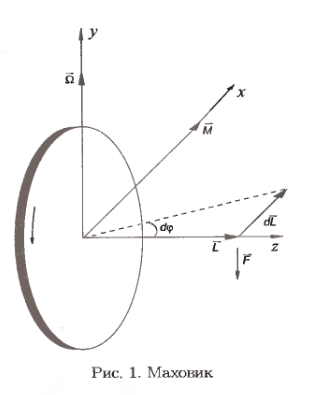
\includegraphics[width=0.40\textwidth]{pic1.png}&
			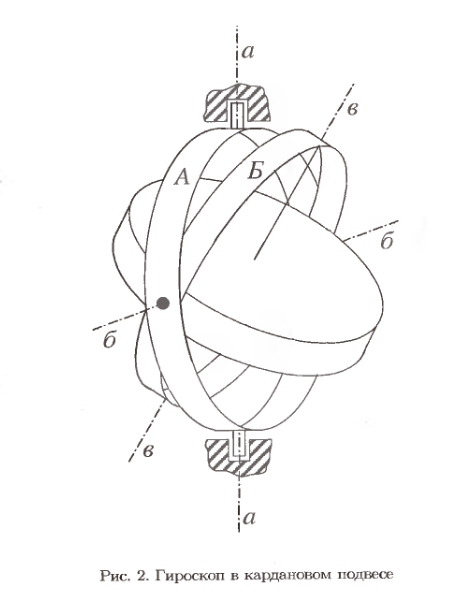
\includegraphics[width=0.40\textwidth]{pic2.png}\\
		\end{array}$
	\end{center}

	 \footnotetext{рисунки взят из учебного пособия "Лабораторный пркатикум по общей физике. Том 1. Механика." }
	Измерение скорости прецессии гироскопа позволяет вычислить угловую скорость вращения его ротора. Расчет производится по формуле:
	
	\begin{equation}
		\Omega = \frac{mgl}{I_z\omega_0},
	\end{equation}
	
	где $m$ -- масса груза, $l$ -- расстояние от центра карданова подвеса до точки крепления груза на оси гироскопа, $I_z$ -- момент инерции гироскопа по его главной оси вращения. $\omega_0$ -- частота его вращения относительно главной оси, $\Omega$ -- частота прецессии.\\
	Момент инерции ротора относительно оси симметрии $I_0$ измеряется по крутильным колебаниям точной копии ротора, подвешиваемой вдоль оси симметрии на десткой проволоке. Период крутильных колебаний $T_0$ зависит от момента инерции $I_0$ и модуля кручения проволоки $f$:
	
	\begin{equation}
		T_0 = 2\pi\sqrt{\frac{I_0}{f}}.
	\end{equation}
	
	Чтобы исключить модуль кручения проволоки, вместо ротора гироскопа к той же проволоке подвешивают цилиндр правильной формы с известными размерами и массой, для которого легко можно вычислить момент инерции $I_\text{ц}$. Для определения момента инерции ротора гироскопа имеем:
	
	\begin{equation}
		I_0 = I_\text{ц}\frac{T_0^2}{T_\text{ц}^2},
		\label{moment}
	\end{equation}
	Здесь $T_\text{ц}$ -- период крутильных колебаний цилиндра.\\
	
	Ниже представлена схема экспериментальной установки (Рис.3\footnotemark)
	\begin{center}
		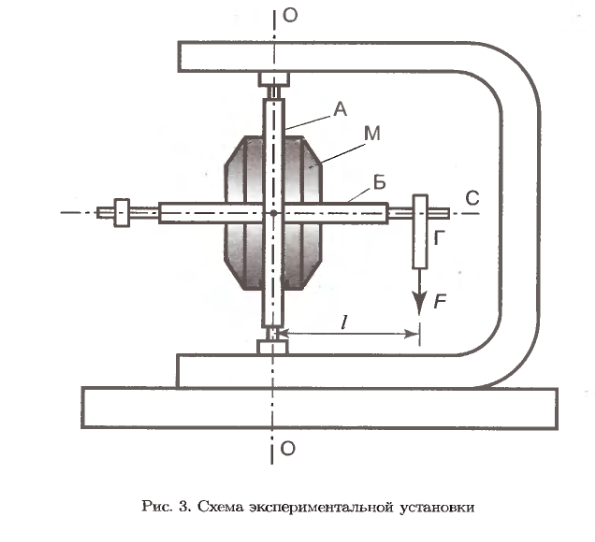
\includegraphics[width=0.65\textwidth]{pic3.png}
	\end{center}
	
	\footnotetext{рисунки взят из учебного пособия "Лабораторный пркатикум по общей физике. Том 1. Механика." }
	Скорость вращения ротора гироскопа можно определить и не прибегая к исследованию прецессии. У используемых в работе гироскопов статор имеет две обмотки, необходимые для быстрой раскрутки гироскопа. В данной работе одну обмотку искользуют для раскрутки гироскопа, а вторую -- для измерения числа оборотов ротора. Ротор электромотора всегда немного намагничен. Вращаясь, он наводит во второй обмотке переменную ЭДС индукции, частота которой равна частоте врещения ротора. Частоту этой ЭДС можно, в частности, измерить по фигурам Лиссажу, получаемым на экране осциллографа, если на один вход подать исследуемую ЭДС, а на другой -- переменное напряжение с хорошо прокалиброванного генератора. При совпадении частот на экране получаем эллипс.
	
	\section{Ход работы}
	Данные для частоты прецессии и опускания гироскопа: $\Omega=\frac{2\pi N}{t}$
	
	\begin{table}[!ht]
		\centering
		\begin{tabular}{|l|l|l|l|l|l|}
			\hline
			№ & $m_\text{цил}$, г & $t_N$, c & N & T, с & $\Omega$, рад/с  \\ \hline
			1 & 341,2 & 148,50 & 5 & 29,70 & 0,212 \\ \hline
			2 & 272,6 & 186,09 & 5 & 37,22 & 0,169 \\ \hline
			3 & 219,2 & 231,18 & 5 & 46,24 & 0,136 \\ \hline
			4 & 178,5 & 283,69 & 5 & 56,74 & 0,111 \\ \hline
			5 & 141,1 & 214,69 & 3 & 71,56 & 0,088 \\ \hline
			6 & 116,4 & 261,75 & 3 & 87,25 & 0,072 \\ \hline
			7 & 92,7 & 217,92 & 2 & 108,96 & 0,058 \\ \hline
			8 & 75,9 & 134,19 & 1 & 134,19 & 0,047 \\ \hline
			9 & 56,5 & 179,75 & 1 & 179,75 & 0,035 \\ \hline
		\end{tabular}
	\end{table}
	
	Построим график зависимости $\Omega(m)$:
	
	\begin{figure}[h!]
		\centering
		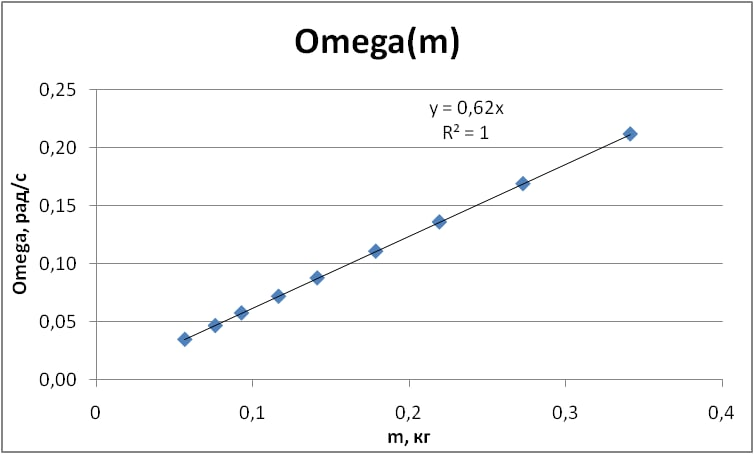
\includegraphics[scale=0.75]{graph1}
		\caption{Зависимость $ \Omega $ от $ m $}
		\label{graph}
	\end{figure}
    
    Из графика получаем коэфициент наклона -- $k = 0,62$, который из формулы для скорости прецессии ($\Omega = \frac{gl}{I_z\omega_0}m$) выражается следующим образом: $k = \frac{gl}{I_z\omega_0}$;
    Из этой формулы выразим искомую частоту вращения ротора: $$\omega_0 = \frac{gl}{I_z k}$$
 
 	Далее найдем момент инерции ротора гироскопа при помощи трифилярного подвеса. По снятым периодам колебания для грузиков с известными параметрами(, а соответсвенно с известными моментами инерции) и для ротора гироскопа определим по формуле \eqref{moment} момент инерции ротора -- $I_0$. Для этого посчитаем момент инерции цилиндра,  с известной нам массой и диаметром: $I_\text{ц} = \dfrac{1}{2}mr^2$, а также моменты инерции для грузиков в форме колечек: $I_\text{гр} = \dfrac{1}{2}m(r^2 + R^2)$   
\begin{table}[!ht]
	\centering
	\begin{tabular}{|l|l|l|l|l|l|l|}
		\hline
		№ & $m_\text{гр}$, г & $I_\text{гр}$, кг*$\text{cм}^2$ & $I_\text{гр} + I_\text{цил}$ , кг*$\text{cм}^2$ & $T_0^2$, $\text{c}^2$ & $T_\text{ц+гр}^2$, $\text{c}^2$ & $I_0$, кг*$\text{cм}^2$ \\ \hline
		1 & 341,2 & 1,75 & 14,08 & 8,38 & 18,69 & 6,31 \\ \hline
		2 & 272,6 & 1,40 & 13,73 & ~ & 18,22 & 6,31 \\ \hline
		3 & 219,2 & 1,13 & 13,45 & ~ & 17,96 & 6,27 \\ \hline
		4 & 178,5 & 0,92 & 13,25 & ~ & 17,64 & 6,29 \\ \hline
		5 & 141,1 & 0,72 & 13,05 & ~ & 17,46 & 6,26 \\ \hline
		6 & 116,4 & 0,60 & 12,93 & ~ & 17,20 & 6,30 \\ \hline
		7 & 92,7 & 0,48 & 12,80 & ~ & 16,86 & 6,36 \\ \hline
		8 & 75,9 & 0,39 & 12,72 & ~ & 16,79 & 6,35 \\ \hline
		9 & 56,5 & 0,29 & 12,62 & ~ & 16,66 & 6,34 \\ \hline
		10 & 1617 & $I_\text{цил}$ = & 12,33 & ~ & 16,55 & 6,24 \\ \hline
	\end{tabular}
\end{table}
	
	Средний момент инерции ротора - $I_\text{ср} = 6,3 \text{ кг}\cdot\text{cм}^2$\\
	Таким образом частота вращения ротора -- $\omega_0 = 2985,9 \text{рад/с} \Leftrightarrow \nu = \frac{\omega_0}{2\pi} = 475\text{ Гц} $
	\section{Погрешности $\Omega$ и $I_0$}
	
	\begin{equation}
		 \sigma_\Omega^\text{сист} = \Omega \varepsilon_T 
	\end{equation}
	
	Каждая частота $\Omega$ с учетом погрешностей:
	\begin{itemize}
		\item $\Omega = (0,2121\pm 0,0002)\text{ }\text{с}^{-1}$,  $\Omega = (0,1694 \pm 0,0002)\text{ }\text{с}^{-1}$
		\item $\Omega = (0,1362 \pm 0,0001)\text{ }\text{с}^{-1}$,  $\Omega = (0,1113 \pm 0,0001)\text{ }\text{с}^{-1}$
		\item $\Omega = (0,0884 \pm 0,0003)\text{ }\text{с}^{-1}$,  $\Omega = (0,0721 \pm 0,0002)\text{ }\text{с}^{-1}$
		\item $\Omega = (0,0583 \pm 0,0005)\text{ }\text{с}^{-1}$,  $\Omega = (0,0472 \pm 0,0006)\text{ }\text{с}^{-1}$
		\item $\Omega = (0,0351 \pm 0,0008)\text{ }\text{с}^{-1}$
	\end{itemize}
	
	Погрешность $\sigma_{I_0}^\text{сист} = I_0\cdot\sqrt{\varepsilon_{I_\text{ц}}^2+ 4\varepsilon_{T_0}^2+ 4\varepsilon_{T_\text{ц}}^2 } \approx 0,1$ кг$\cdot \text{cм}^2$,\\ $$\sigma_{I_0}^\text{случ}=  \sqrt{\frac{1}{n(n-1)} \sum_{i=1}^{n}({I_0}_i - \overline{{I_0}})^2} \approx 0,01 \text{кг}\cdot \text{cм}^2$$  
	$\sigma_{I_0} = \sqrt{ \sigma_\text{случ}^2 + \sigma_\text{сист}^2}$,   значит $I_0 = (6,30\pm 0,1)$ кг$\cdot \text{cм}^2$, $\varepsilon_{I_0} = 1,6\%$
	
\section{Вывод}
	Частота вращения ротора измереная с помощью осцилографа  -- $\nu = (400,1 \pm 0,5)	$, причем при выходе из этого диапазона фигура Лиссажу, образованная кратными сигналами с генератора и гироскопа, исчезает. Экспериментально полученное значение частоты вращения ротора -- $\nu = (475 \pm 8)\text{ Гц} $, $\varepsilon_{\nu} = 1,7\%$. Значения значительно расходятся(10$\sigma_\nu$), это может быть связано с грубой ошибкой при снятии измерений. 
\section{Оценка момента силы трения}

	Для оценки момента силы трения снимем понижение оси за 6 периодов вынужденной прецессии (с грузом массой - $m =  272,2 \text{ г}$) -- $t = 223,3 \pm 0,1 \text{ с}$ -- снижение до вертикального положения равно $\Delta H = 1,8 \pm {0,1} \text{ см.}$ при длине "рычага" в $l = 12,8 \pm {0,1} \text{см}$.\\ 
	Тогда он опустился на $\varphi = \arcsin(\frac{\Delta H}{l})=0,141 \text{рад}$,\\ $\sigma_\varphi=\varphi\sqrt{(\frac{\sigma_{\Delta H}}{\Delta H})^2+(\frac{\sigma_ l}{l})^2}=8\cdot10^{-3}\text{рад}$.\\
	Тогда момент силы трения -- $M_{\text{тр}}=\frac{\varphi}{T}\cdot I\omega = 1,19 \text{мН}$,\\ $\sigma_{M_{\text{тр}}} = \sigma_{M_{\text{тр}}}\sqrt{(\frac{\sigma_\varphi}{\varphi})^2+(\frac{\sigma_T}{T})^2 + (\frac{\sigma_I}{I})^2+(\frac{\sigma_\omega}{\omega})^2} = 0,08\text{мН}$, таким образом  $\varepsilon_{M_{\text{тр}}} = 6,8\%$ 

	
\end{document}